\documentclass[aps,prl,groupaddress, twocolumn]{revtex4-1}  % chktex 8
\usepackage{filecontents}
%\usepackage{subcaption}  %% don't use subcaption. It's incompatible with revtex...
\usepackage{amsmath}
\usepackage{amsfonts}
\usepackage{natbib}
\usepackage{multirow}
\usepackage{float}
\usepackage{graphicx}
%\usepackage{subfigure}
\usepackage{xcolor}
%\usepackage{cleveref}
\usepackage[colorlinks,urlcolor=blue]{hyperref}
\usepackage{braket}
\raggedbottom%
% Customed commands
\DeclareMathOperator{\erf}{Erf}
\newcommand{\obrt}{\frac{1}{\sqrt{2}}}
\newcommand{\lp}{\left(}  % chktex 9
\newcommand{\rp}{\right)}  % chktex 9
\newcommand{\diff}{\mathrm{d}}
\newcommand{\ham}{\hat{\mathcal{H}}}
\newcommand{\p}{\hat{p}}
\newcommand{\num}{\hat{N}}
\newcommand{\rr}{\mathbf{r}}
\newcommand{\fact}[1]{#1!}
\newcommand{\abs}[1]{\left\vert{#1}\right\vert}
\newcommand{\Abs}[1]{\left\Vert{#1}\right\Vert}
%\newcommand{\bra}[1]{\langle #1 \vert}
%\newcommand{\ket}[1]{\vert #1 \rangle}
\newcommand{\newtext}[1]{{\color{red}#1}}
\newcommand{\ie}{\emph{i.e. }}
\newcommand{\viz}{\emph{viz.}}
\newcommand{\eg}{\emph{eg. }}
\newcommand{\via}{\emph{via }}
% Textbody
\begin{document}
\title{Dipole approximation to van der Waals interactions insufficient for large systems}	

\author{Mainak Sadhukhan}
\affiliation{Physics and Materials Science Research Unit, University of Luxembourg, L-1511 Luxembourg}
\author{Yasmine Al-Hamdani}
\affiliation{Physics and Materials Science Research Unit, University of Luxembourg, L-1511 Luxembourg}
\author{Martin St\"{o}hr}
\affiliation{Physics and Materials Science Research Unit, University of Luxembourg, L-1511 Luxembourg}
\author{Jan Hermann}
\affiliation{Physics and Materials Science Research Unit, University of Luxembourg, L-1511 Luxembourg}
\author{Alexandre Tkatchenko}
\email{alexandre.tkatchenko@uni.lu}
\affiliation{Physics and Materials Science Research Unit, University of Luxembourg, L-1511 Luxembourg}
\date{}





%\begin{document} 


\begin{abstract}
Long-range repulsive contributions to the interactions between confined molecules have been evidenced by a number of experiments and recently also demonstrated theoretically. This physical repulsive interaction has been missing from van der Waals (vdW) approximations in density functional theory (DFT) methods to date. Given the tendency of vdW-inclusive methods in DFT to overbind confined systems, the inclusion of the first-order full Coulomb interaction to the many-body dispersion (MBD) method is expected to alleviate overbinding. We develop an approach to include this term in combination with the MBD formalism, such that the well-established S66 benchmark data set is computed with an accuracy of xx kJ/mol. This method is then applied to supramolecular confined systems such as the prototypical buckyball-catcher and also buckyball-ring systems. We find that the effect of the long-range repulsive interaction is significant in the confined systems and should be included to make accurate and physically coherent predictions. 
\end{abstract}
\maketitle

%%\section{Introduction}
% \textit{Motivation: general beyond-dipole correction, which, under confinement, can qualitatively alter the long-range behaviour. Then we can state afterwards: first we look at the general case of vdW-dimers/complexes and then we turn to(wards) confinement.}

\section*{Introduction} 
Long-range dispersion interactions between atoms and molecules, though typically characterized as ``weak'', underpin a great deal of physical and chemical behavior in biological and material science. The intricacies of quantum mechanical electron density fluctuations, in particular, is an intense area of research that is driven to a great extent by the challenge of capturing its many-body nature. As such, the vast majority of computational studies to date are not able to fully account for the many-body dispersion interactions that arise from electron density fluctuations. It is typically envisaged that a dipole-coupled approximation to the dispersion interaction is sufficient to accurately predict properties of interest, such as binding energies and geometries. However, this notion is increasingly disputed as the missing physics in the most widely used computational methods continues to stand in the way of understanding \textit{state-of-the-art} experimental phenomena. 
% Quantum mechanical electron fluctuations naturally present a many-body problem and are therefore, the source of ongoing challenges.
% Experiments show that simulations are still a long way from providing definitive explanations to observed phenomena. 

For example, Secchi \textit{et al.} found that water flows ultra-fast through narrow carbon nanotubes (CNT), but not through boron nitride nanotubes (BNNT)~\cite{secchi2016massive}. In this regard, theorists are still working towards satisfactory modeling of this effect and capturing the underlying physical interactions~\cite{Michaelides2016,Kannam2013,Striolo2016,Mattia2015266}. In a similar vein, the spatial separation and ordering of large polarizable molecules on metal surfaces~\cite{Wagner2010,Thussing2016}, salient in organic thin films for organic electronics, highlights gaps in common modelling approaches. For instance, Wagner~\textit{et al.} showed that large aromatic molecules organize into highly ordered arrays at high coverage on Au(111)~\cite{Wagner2010}. Interestingly, the authors rationalize their findings using repulsive, Coulombic intermolecular interactions, induced by screening from the metal.  % chktex 36

%Our work here elaborates on the physical interactions that are indicated in the aforementioned experiments, using a fundamental theoretical basis which we use to predict a number of complexes.

The experimental examples of Secchi~\textit{et al.} and Wagner~\textit{et al.} are confined systems. Confinement in general is prevalent, \textit{e.g.} a molecule adsorbed on a surface is quasi-3D confined; a molecule in a narrow nanotube is quasi-1D confined; and a molecule between two sheets is quasi-2D confined. Dispersion interactions play a key role in confined systems, but are challenging to compute with accurate quantum mechanical methods due to the typical size and complexity of confined systems. The complexity of confined systems, in particular, calls for a complete description of Coulombic interactions between fluctuating electron densities, to fully account for all dynamic correlation. However, this is practically an insurmountable task for anything beyond a few atoms. One effective method of predicting larger systems is to use a perturbative approach to go beyond the simple dipole-coupled approximation. As we describe hereafter, by accounting for higher multipoles in a perturbative approach, we better approximate the quantum behavior of fluctuating charge densities. 

\begin{figure}[h]
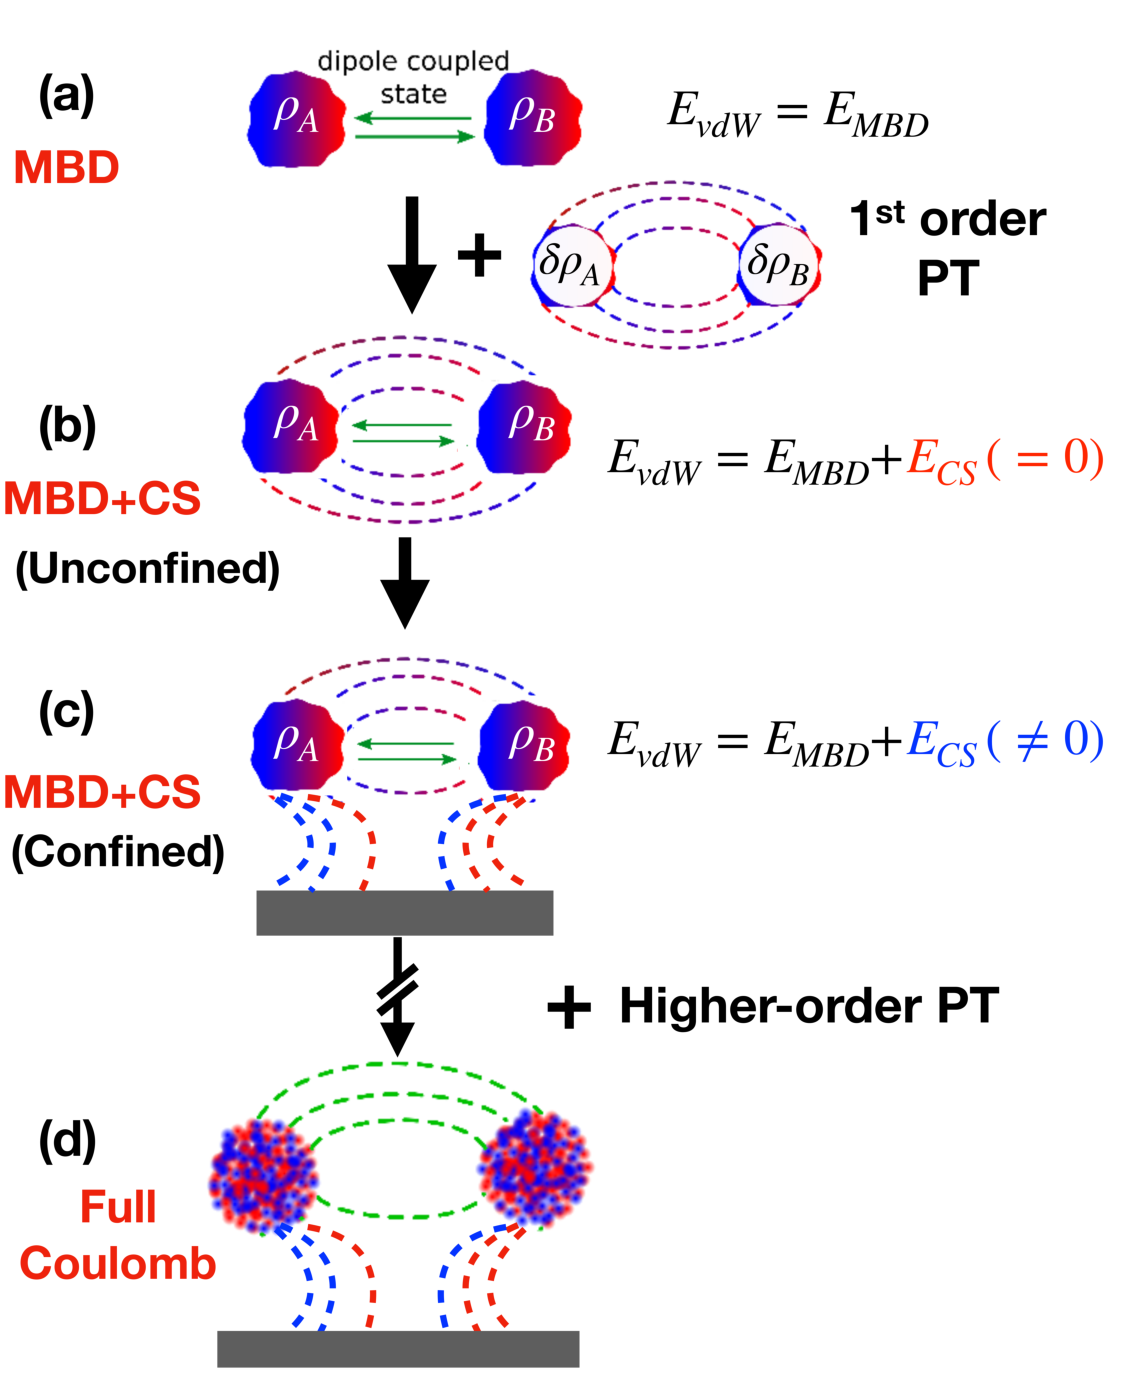
\includegraphics[scale=0.45]{Plots/Schematic_new.pdf}
\caption{\textbf{Schematic representation of Coulomb singles correction:} (a) Green arrows represent dipole-coupling between electronic fragments. 1$^{\rm st}$-order perturbation theory (PT) captures full-Coulomb singles interaction energy, $E_{\rm CS}$, depicted by field lines. (b) 1$^{\rm st}$-order correction vanishes in 3D isotropic vacuum due to symmetry reasons, \textit{i.e.} $E_{\rm CS} = 0$. (c) Under rotational symmetry-breaking confinement, electric field-lines between electronic fragments get deformed leading to $E_{CS} \neq 0$. (d) Further inclusion of higher-order PT leads to full Coulomb-coupled van der Waals interaction.}\label{fig:schematic}
\end{figure}
% conceptual introduction into the physics of CS
%Coulomb interactions between spontaneously fluctuating electron densities give rise to well-known van der Waals interactions. 

While charge density fluctuations are purely quantum-mechanical, they can be visualized as instantaneous deformations of electron density. In 3D isotropic vacuum, the longest range interactions between these electronic fluctuations is dipolar in nature, which gives rise to the famous attractive London dispersion interaction. This observation, however, led to the widespread assumption that the long-range interaction between two polarizable electron densities, without any permanent moment, is always attractive and mediated by dipole-coupling. We can, however, extend the description by perturbatively adding the remaining terms of the Coulomb interaction on the dipole-coupled states\cite{sadhukhan_prl_2017}. Taking two electron densities $\rho_A$ and $\rho_B$ (Fig.~\ref{fig:schematic}a) and applying dipole-coupling between them, the van der Waals interaction energy ($E_{vdW}$) is described only by dipole-coupled theory in this way. The many-body dispersion (MBD) method that yields the MBD energy ($E_{\rm MBD}$), as shown at the top of Fig.~\ref{fig:schematic}a, is one such method. As a result of dipole-coupling however, the electron densities, $\rho_A$ and $\rho_B$, change by $\delta \rho_A$ and $\delta \rho_B$, respectively. The first order beyond-dipole perturbation describes the Coulomb interaction, represented by electric field-lines (dashed lines) in Fig.~\ref{fig:schematic}, between $\delta \rho_A$ and $\delta \rho_B$. Formal comparison to post Hartree--Fock electronic structure theories indicate that this interaction resembles that between singly excited fragments (\textit{i.e.} the dipolar states in Fig.~\ref{fig:schematic}). This resemblance prompted us to name this interaction energy the \textit{Coulomb singles} ($E_{\rm CS}$) interaction energy. For a system in 3D isotropic vacuum (unconfined), $E_{\rm CS}$ vanishes in the long-range due to the symmetry between the incoming and outgoing electric field-lines (schematically shown in Fig.~\ref{fig:schematic}b). However, under confinement which breaks 3D isotropic symmetry, $E_{\rm CS}$ is non-zero (see Fig.~\ref{fig:schematic}c) and therefore contributes significantly to $E_{vdW}$. Experimental or theoretical estimation of van der Waals interaction energies for such large confined systems has been a long-standing challenge and has only become feasible in recent years. With recently available reference interaction energies, we are closer to defining the missing components of van der Waals interactions in our theoretical models. In future, higher-order corrections will eventually bring the theoretical description even closer to full Coulomb-coupling between fluctuating electron densities (illustrated in Fig.~\ref{fig:schematic}d).


%the role of 1st order term versus higher orders
Coulomb singles can comprise an appreciable part of the overall picture of long-range interactions in physical systems. We incorporate this interaction in a practicable, fully atomistic, MBD approach in DFT and model a range of materials, from unconfined small molecular dimers to large supramolecular confined materials. In doing so, we demonstrate that there can be an intricate balance between attractive and repulsive long-range terms when Coulomb singles are included; such that under confinement long-range repulsion can become dominant at length scales beyond several \r{A}ngstr\"{o}ms of intermolecular separation. What is more, we show that Coulomb singles are entirely befitting to all forms of matter, with a varying degree of impact, as would be expected. 

\section*{Coulomb corrections for small molecular dimers}
We begin by applying the first order perturbation term in the S66 molecular data set of small, unconfined dimers. A consistent approach to incorporate the Coulomb singles with the MBD approach is referred to as MBD+CS and is constructed by analyzing the first-order perturbation theory (PT) correction for small molecular dimers as contained in the S66 database~\cite{s66X8_database}.
%(Fig.~\ref{fig:s66}). 
For such systems, semi-local or hybrid density functional approximations in conjunction with the MBD formalism are designed to provide excellent agreement with accurate reference results from coupled cluster with single, double, and perturbative triple excitations (CCSD(T)) calculations~\cite{Tkatchenko2012}.  % chktex  36
%, shown in red dots in Fig.~\ref{fig:s66}(A). 
The S66 dimers are close approximations to van der Waals dimers in 3D isotropic vacuum and in accordance with Fig.~\ref{fig:schematic} we expect minuscule first-order Coulomb corrections in these cases.
%Fig.~\ref{fig:s66}(A) indeed shows that
Indeed, we find that the CS contributions for all systems in S66 are very small and they can have both positive as well as negative values (see the Supplementary Material for more information). As a result, addition of CS barely affects PBE+MBD binding energies for small organic dimers.
In the next sections, we use MBD+CS to compute supramolecular host-guest complexes and confined Xe atoms in capped CNTs. These larger confined systems reveal the impact of Coulomb singles on binding energies, as well as the length-scale and character of the repulsive long-range interaction that manifests. 

%In the next sections we use MBD+CS to compute supramolecular host-guest complexes and confined Xe atoms in CNTs. In doing so, the accuracy of MBD+CS is assessed with respect to experimental and wavefunction-based reference information. Furthermore, we establish the length scale and character of the long-range repulsive interaction that manifests between CNT confined Xe atoms. 
%A general discussion and summary will be given and finally, the theoretical basis of the Coulomb singles and how it is combined with the MBD approach is given. There also, the computational methods are presented along with details of the molecular systems computed.

\section*{Coulomb corrections for host-guest complexes}
Host-guest molecular systems are significantly more complex than those of S66 dimers, but are still tractable with accurate benchmark methods such diffusion quantum Monte Carlo (DQMC). Here, we first ascertain the impact of CS on the interaction energies of host-guest complexes and demonstrate the accuracy of PBE0+MBD+CS with respect to DQMC reference interaction energies. In addition, a connection might be expected between geometrical factors (\textit{e.g.} asymmetry and steric effects) and the magnitude of CS contributions. To this end, we analyze this possible connection in geometrically similar host-guest complexes and arrive at important insights on the quantum mechanical nature of $E_{\rm CS}$.     

\subsection*{Interaction energies of two host-guest complexes}

The accurate prediction of interaction energies for non-covalently bound materials is an ongoing challenge for researchers and workhorse DFT methods are at the forefront of development efforts. The complex balance of intermolecular interactions is particularly challenging to predict and what is more, the target accuracy is generally in the range of a few kJ/mol in interaction energies. Our approach to better accuracy is to improve the physical basis of theoretical methods---here, by incorporating the CS contributions. 
Fig.~\ref{fig:flagshipsystems} shows two select examples of host-guest complexes. For both systems, the guest molecule is a C$_{70}$-fullerene (buckyball) while the host is either [6]-cycloparaphenyleneacetylene (6-CPPA, Fig.~\ref{fig:flagshipsystems} left) or the ``catcher'' molecule (Fig.~\ref{fig:flagshipsystems} right)~\cite{s12l_2013}. In the framework of Fig.~\ref{fig:schematic}, the host molecule serves as both confinement and interaction partner. The extensive 6-CPPA and catcher molecules provide a different confining environment for the buckyball by virtue of their structure. We therefore focus on these systems to showcase the contribution of CS in confined systems. 
\begin{figure}[htp!]
\centering
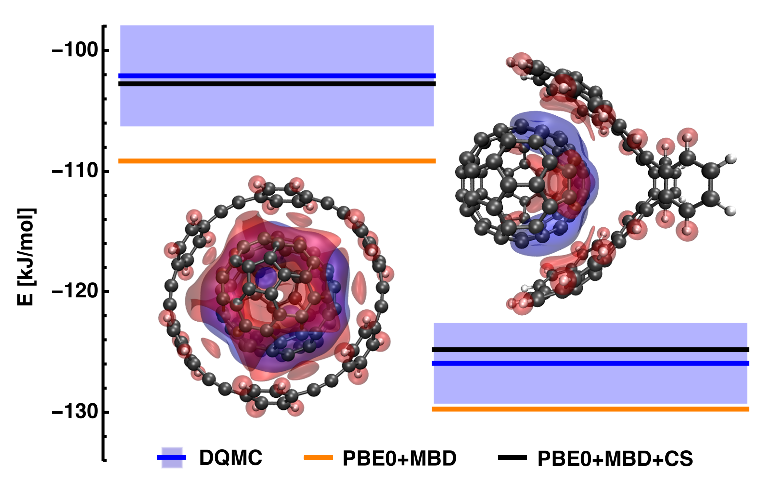
\includegraphics[scale=0.68]{Plots/S12L4b.eps}
\caption{Binding energies of C$_{\bf 70}$ in 6-CPPA (left) and in the ``buckyball-catcher'' (right):
PBE0+MBD results (orange), DQMC reference (blue line, error bars shown as boxes), PBE0+MBD including Coulomb singles contribution (black line).
DQMC reference data taken from Ref.~\cite{hermann_ncomm2017}.
The depiction of the complexes also includes isosurfaces at $\pm$0.003 of the change in the density of electronic fluctuations with respect to the isolated monomers (red: decrease, blue: increase).
}\label{fig:flagshipsystems}
\end{figure}

\begin{figure*}[hbtp]
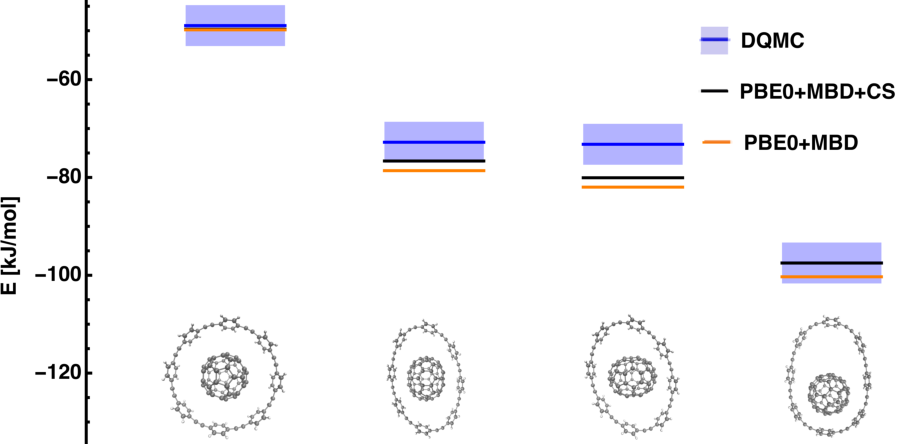
\includegraphics[scale=1.]{Plots/Rings_new.pdf}
\caption{\textbf{CS contributions for ring-C$_{70}$ complexes.} Comparison of binding energies for different ring-C$_{70}$ host-guest complexes (R1-R4).The blue solid lines and light blue bars represent benchmark DQMC binding energies and corresponding stochastic errors. Orange and black lines represent PBE0+MBD and PBE0+MBD+CS binding energies. The hosts for R1--R4 are 8-CPPA rings. The CS contribution is significant and changes across the systems.}\label{fig:rings}
\end{figure*}

Within the dipole approximation, it has already been shown that many-body effects play an important role for the description of binding energies in such guest-host complexes~\cite{hermann_ncomm2017}. Here, we show that also beyond-dipole interactions, in the form of CS, have a significant effect and that inclusion of CS to PBE0+MBD yields excellent agreement with reference results from DQMC\@. The CS contribution for C$_{70}$ in 6-CPPA and in the buckyball-catcher are 6.39~kJ/mol and 4.92~kJ/mol, respectively. Considering our findings for the S66 data set above, this clearly highlights the importance of CS corrections under confinement, \textit{i.e.} once the 3D vacuum isotropy is substantially perturbed. It is important to note here that the relative contributions of CS to the total binding energies for these systems are 6.22\% and 3.94\%, respectively. 

These different contributions can be interpreted in terms of the physics of the dipole-coupled state, which represents the starting point (unperturbed state) for the calculation of the CS contribution by means of PT\@.
One such characteristic is the density of electronic fluctuations in the dipole-coupled state (\textit{i.e.} the ``MBD density''), which can be obtained as the expectation value of the charge density operator via the MBD wave function, $\Psi_{\rm MBD}$ (\textit{vide infra}).
Looking at the host-guest interaction, we analyze the difference in the density of electron fluctuations with respect to the isolated monomers.
This gives a measure for how much the MBD density is deformed upon interaction and therefore, forms a connection between confinement and electronic fluctuations or polarizability. 
The density difference shown in Fig.~\ref{fig:flagshipsystems}%, where red regions indicate a decrease and blue regions an increase in the density.
%As can be seen from this depiction, 
shows the density of electronic fluctuations for C$_{70}$ in 6-CPPA is strongly compressed into the plane of 6-CPPA, on the guest and the host molecules.
We furthermore found that the overall displaced charge, \textit{i.e.} the integral over the density difference, can serve as a descriptor for the CS contribution to the interaction energy:
With increasing displaced charge, we observe an increased CS contribution to the interaction energy. We would like to point out that this also applies to the remaining systems considered below.
Hence, the electronic properties obtained for a dipole-coupled state can serve as a qualitative \emph{rule-of-thumb} to estimate the CS energy.
% \textcolor{red}{\textbf{later: also explain this in terms of field lines of CS as in Fig.~\ref{fig:schematic}. (should be easily accessible in current framework of calculating CS...)}}

\subsection*{Asymmetry and Coulomb singles in host-guest complexes}
Naturally, one might quantify confinement in terms of the (molecular) geometry. Among other measures, the asymmetry of the system and the proximity of atoms or subsystems represent common descriptors. To explore such connections between $E_{\rm CS}$ and geometrical features, we additionally analyze a class of geometrically similar ring--C$_{70}$ complexes as depicted in Fig.~\ref{fig:rings}: The first four complexes are C$_{70}$ hosted by four different conformations of 8-CPPA and the last is a second configuration of C$_{70}$ in 6-CPPA with the fullerene being situated partly outside the host (dubbed ``tilted conformation'' in Ref.~\cite{hermann_ncomm2017}). Also in this case, PBE0+MBD has been shown to already provide reasonably accurate binding energies with respect to DQMC~\cite{hermann_ncomm2017}. As can be seen from Fig.~\ref{fig:rings}, addition of the CS contribution to PBE0+MBD, again, improves the obtained binding energies in all cases.

Despite the molecular similarities, the individual CS contributions vary significantly also across these systems.
The displaced charge with respect to isolated monomers introduced above as a measure for the confinement of the electronic response, thereby, again resembles the general trend of the CS energy, which further strengthens the connection between electronic confinement and the CS contribution.
\begin{figure*}[htp]
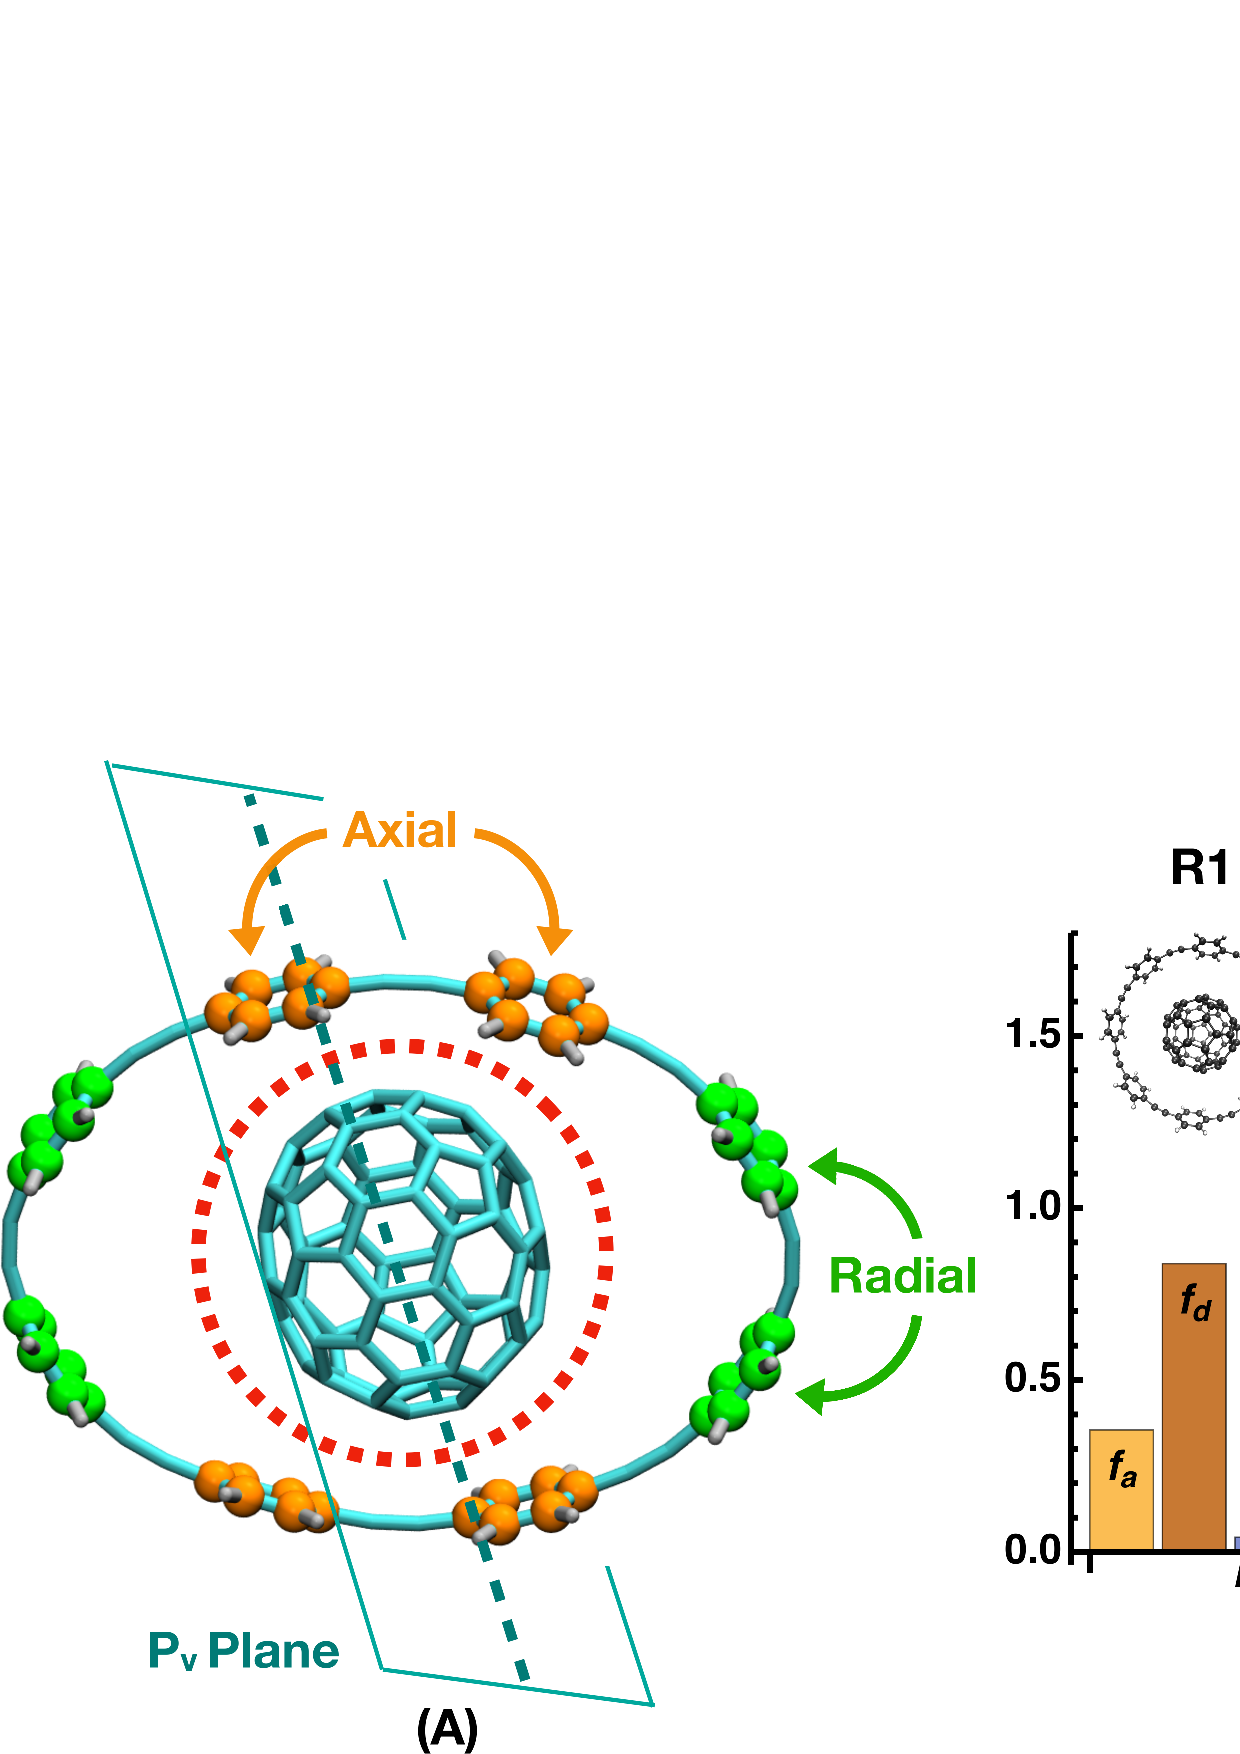
\includegraphics[scale=0.5]{Plots/Analysis8Rings.pdf}
\caption{\textbf{Correlation between structural features of C$_{70}$ in 8-CPPA and corresponding contribution of \emph{Coulomb singles}.} (A): Definition of ``axial'' and ``radial'' phenyl units of 8-CPPA via P$_v$ plane. (B): Measure for axial-radial asymmetry ($f_a$), proximity measure ($f_d$), and \emph{Coulomb singles} contribution to binding energy (all values normalized to results for R4).}\label{fig:analysis_rings}
\end{figure*}

In order to investigate connections between the molecular structure and general trends in the CS contribution, we define two geometrical measures:
One for proximity ($f_d$), which is given by the sum of inverse distances between the atoms of the fullerene and the CPPA-host, and one for the asymmetry of the system ($f_a$).
For the latter, we first define an axis along the elongated direction of C$_{70}$ and then span a plane along that axis, perpendicular to the CPPA-ring, labeled as P$_v$ in Fig.~\ref{fig:analysis_rings}A.
The four phenyl units closest to this plane are considered as ``axial'' and the remaining four as ``radial'', see Fig.~\ref{fig:analysis_rings}A.
Based on this classification, we define ``axial vicinity'' ($A_{\parallel}$) and ``radial vicinity'' ($A_{\perp}$) by summing the inverse distances between all fullerene atoms and atoms of the corresponding ``axial'' and ``radial'' phenyl rings, respectively.
Our measure for (axial-radial) asymmetry is then given by $f_a = (A_{\parallel} - A_{\perp})/(A_{\parallel} + A_{\perp})$. Fig.~\ref{fig:analysis_rings}B summarizes the results for the proximity and asymmetry measure and the CS energy normalized to R4.
It is clear that, in principle, proximity plays a certain role for electronic confinement (\textit{cf.} proximity and CS contributions for C$_{70}$ in 6-CPPA and R1). As can be seen from our more detailed analysis in Fig.~\ref{fig:analysis_rings} however, purely geometrical considerations do not suffice to capture the trends in $E_{\rm CS}$: The proximity measure, $f_d$, is insensitive to the relevant changes and remains almost constant among all studied systems, while the CS contribution varies significantly.
Furthermore, the asymmetry measure, $f_a$, turned out to show no correlation with the results for $E_{\rm CS}$ (see R3 versus R4 in Fig.~\ref{fig:analysis_rings}).
Thus, also a pairwise description of asymmetry between atomic positions is insufficient to predict the qualitative trend of the contribution of CS\@.
The failure to capture the behaviour of $E_{\rm CS}$ in terms of simple geometrical characteristics, stems from the fact that the CS contribution is a purely quantum-mechanical effect arising from beyond-dipole interactions of electronic fluctuations, which show a far-from-trivial dependence on a system's geometrical features.\\

\section*{Impact of Coulomb singles in capped carbon nanotubes}
\begin{figure*}[hbtp]
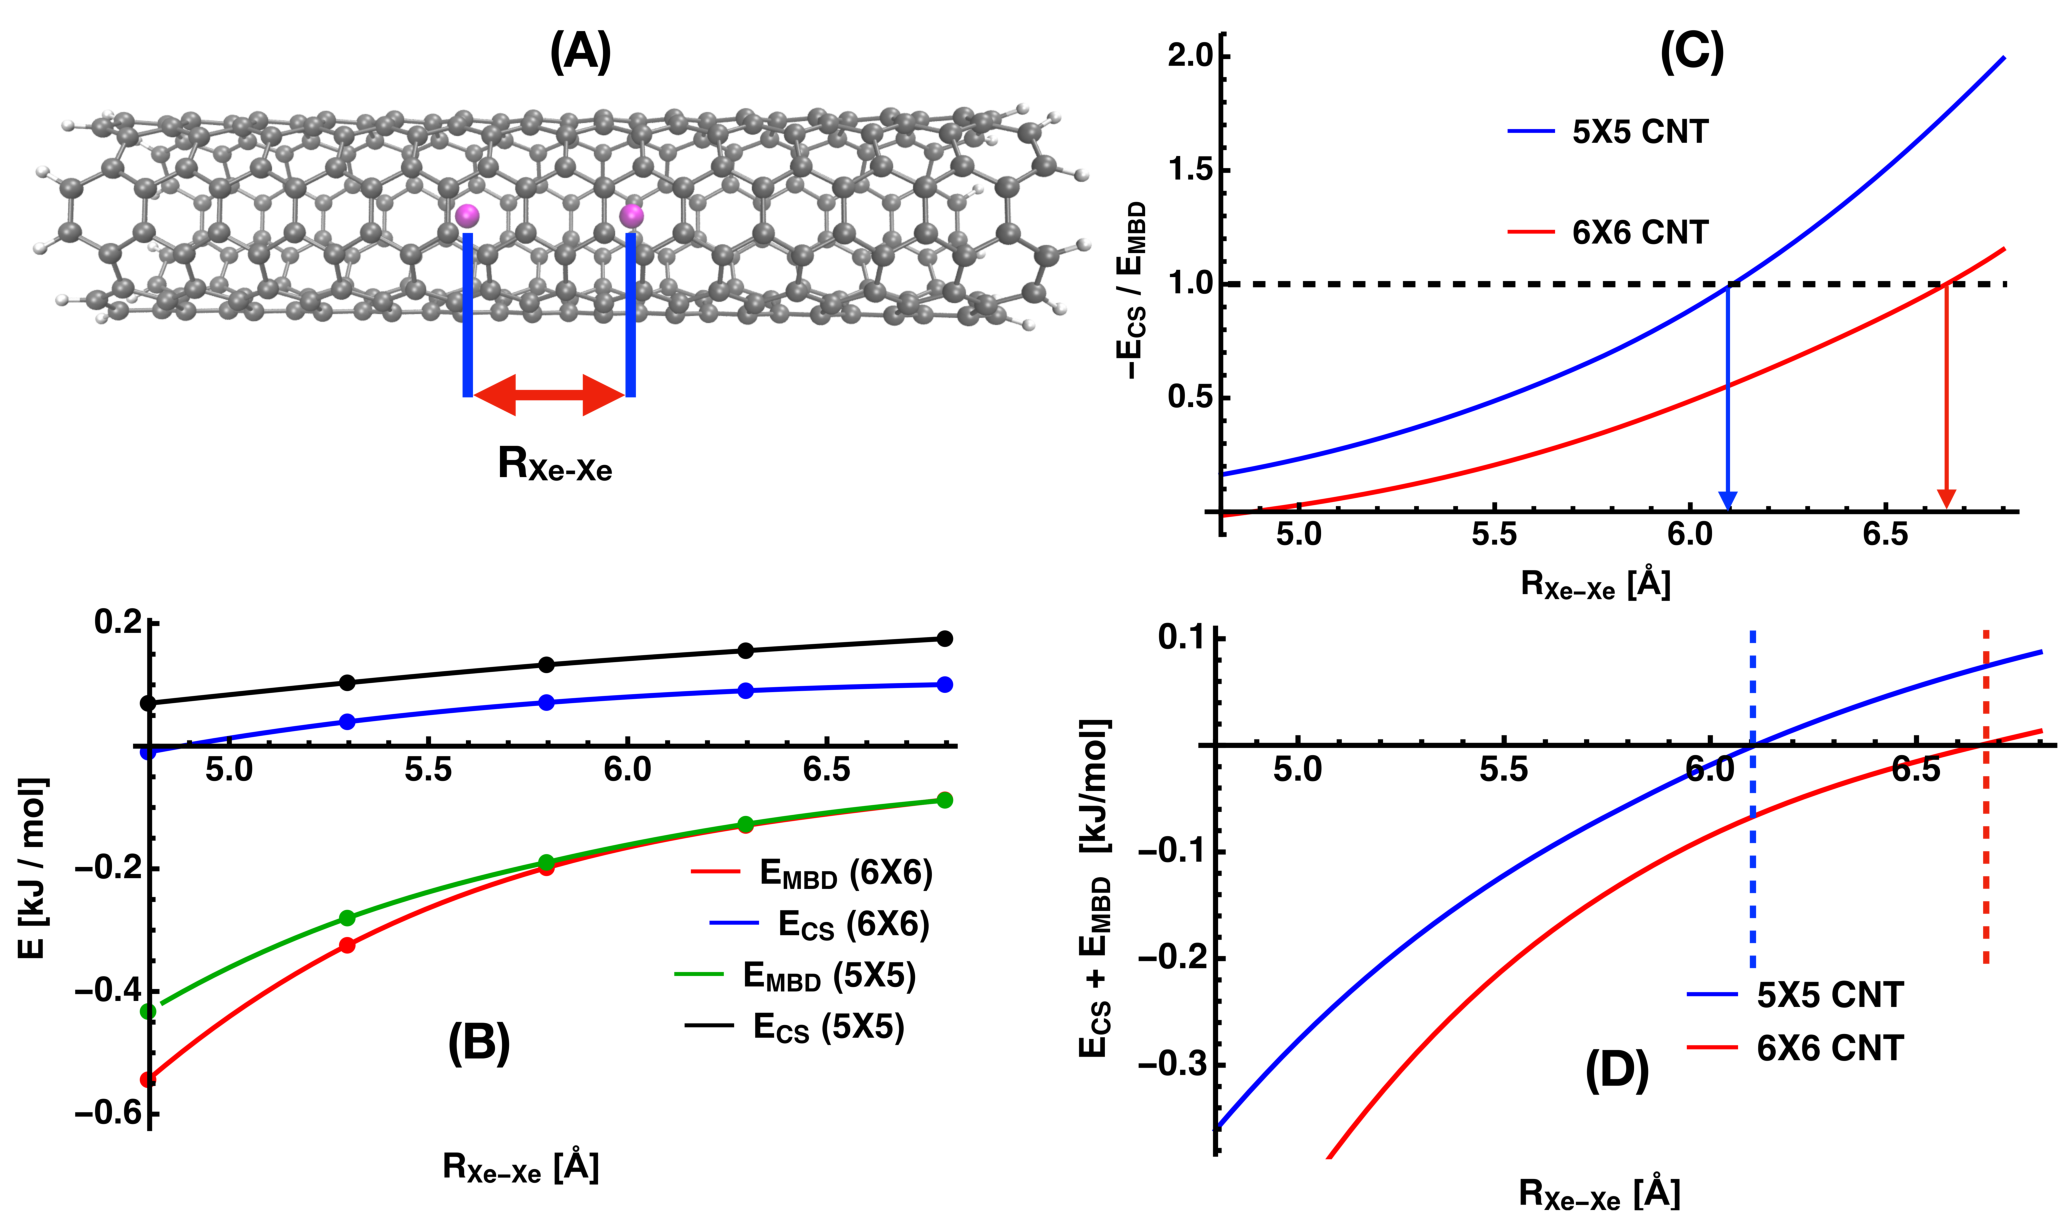
\includegraphics[scale=0.5, width=\textwidth]{Plots/CNTplots.pdf}
\caption{\textbf{Variation of MBD and CS contributions with Xe-Xe distance} (A) Two Xe atoms (mauve) encapsulated by the carbon nanotube. (B) Variation of $E_{\rm MBD}$ and $E_{\rm CS}$ with the change of $R_{Xe-Xe}$. The black and blue lines are $E_{\rm CS}$ for $5 \times 5$ and $6 \times 6$ CNTs. The difference between them is prominent for all distances. Green and red lines are $E_{\rm MBD}$ for $5 \times 5$ and $6 \times 6$ CNTs which converges more quickly than $E_{\rm CS}$. (C) The ratio of $-E_{CS}$ and $E_{\rm MBD}$ represent the balance between them with $R_{Xe-Xe}$. Blue and red lines represent the ratio for $5\times5$ and $6\times6$ CNTs. In shorter distance, the attractive $E_{\rm MBD}$ dominates while in longer distance repulsive $E_{\rm CS}$ supersedes the attraction. The threshold interatomic distance at which this inflection occurs is smaller for the narrower CNT (blue arrow) and longer for wider CNT (red arrow). (D) The cumulative van der Waals interaction changes from attractive to repulsive with increasing $R_{Xe-Xe}$ for both nanotube radii.}\label{fig:CNT}
\end{figure*}
Having established the importance of $E_{\rm CS}$ for confined host-guest systems, we now employ our methodology to investigate the effects of confinement for Xe dimer inside carbon nanotubes (CNT). We will be investigating how the confinement changes the relative importance of Coulomb corrections on dipole coupled van der Waals interactions. Xe does not posses a permanent multipole and has a considerably large polarizability. As a result, the Xe-Xe interaction is purely van der Waals. 
%carbon nanotube's structure and its connection to polarizability
%Carbon nanotubes, in principle, can be created by folding a 2D graphene sheet. 
%Depending on the way of folding, 

CNTs can be distinguished by their chiral vector $\mathbf{R}=m \mathbf{a}_1 +n \mathbf{a}_2 $. 
%Here $\mathbf{a}_1$ and $\mathbf{a}_2$ are unit cell vectors for 2D graphene sheet. Therefore, the atomic arrangement of CNTs, and hence their electronic properties, are dependent on the integer pair $m$ and $n$. 
Armchair CNTs, with $m=n$, are metallic in nature by virtue of their delocalized electronic states. Since, the CS contribution becomes significant in the presence of metallic screening\cite{sadhukhan_prl_2017}, we analyze the Xe-Xe binding energy inside two armchair, hydrogen-capped CNTs with $m = n = 5$ and $m = n = 6$. The diameters of $5\times5$ and $6\times6$ CNTs are 6.78 \AA\ and 81.3 \AA, respectively. The length of these nanotubes is 30 \AA, which is long enough to avoid significant edge-effects and to serve as a model for a periodic CNT\@. The binding energies of Xe dimer inside a nanotube is calculated as $E_{Xe-Xe} = E_{Xe_2+CNT}+E_{CNT} - 2 E_{Xe+CNT}$, where $E_{Xe_2+CNT}$, $E_{Xe+CNT}$ and $E_{CNT}$ are the energies of Xe dimer hosted by a CNT, one Xe atom hosted by a CNT, and a bare CNT, respectively. 

%desription of results of Xe dimer inside CNTs
Fig.~\ref{fig:CNT} summarizes the effect of the confining potential of capped CNT on the Xe dimer binding energy. We focus on the variation of dipole-coupled MBD and corresponding CS contributions as a function of the inter-Xe distance $R_{Xe-Xe}$ (see Fig.~\ref{fig:CNT}A). Fig.~\ref{fig:CNT}B demonstrates these energy components for CNTs of both diameters. Note that $E_{\rm MBD}$ for both CNTs converge to an asymptotic value while $E_{\rm CS}$ does not. Clearly, $E_{\rm CS}$ is much more sensitive to the confining effects of CNT compared to the $E_{\rm MBD}$. In 3D isotropic vacuum, Xe dimer equilibrium distance and binding energy are 4.36 \AA\ and 2.35 kJ/mol, respectively\cite{Jerabek_2017}. The much smaller magnitude of Xe-Xe interaction energies inside the CNTs demonstrates a strong destabilizing effect on the Xe dimer binding energy as a result of the confining CNT\@. As expected, the Xe dimer inside the $6\times6$ CNT is less affected by the vicinity of the CNT wall and is more stabilized. Similarly, the CS interaction increases with narrower CNT\@. Evidently, the CS contribution decays at much longer interatomic distance compared to the MBD energy. The power-law fitting of these two energies (see SI) show that the MBD interaction energy can be fitted reasonably with $R_{Xe-Xe}^{-6}$ and $R_{Xe-Xe}^{-12}$. However, one needs significantly larger number of power-law terms to fit $E_{\rm CS}$. This is indicative of the longer-range nature of $E_{\rm CS}$. These results, therefore, support our previous prediction regarding the length-scale of CS\cite{sadhukhan_prl_2017, sadhukhan_prl_reply2018}. 

%balance of attraction and repulsion
To explore the balance between repulsive $E_{\rm CS}$ and attractive $E_{\rm MBD}$ more clearly we plot the ratio of absolute value of them as a function of $R_{Xe-Xe}$ in Fig.~\ref{fig:CNT}C. We see clearly that for both CNT diameters, the ratio increases with $R_{Xe-Xe}$ and crosses 1.0, which signifies that the $E_{\rm CS}$ eventually supersedes $E_{\rm MBD}$. Therefore, in longer range $E_{\rm CS}$ becomes the dominant contribution. This is remarkable considering the previous \textit{status quo} that in the long-range, the van der Waals interaction is always be attractive. This is the first time we see that the longer range van der Waals interaction is actually repulsive under confinement. As evident from the divergent trend of the ratios for these two nanotubes, the $E_{\rm CS}$ contribution overrides long-range attraction more drastically for narrower nanotube. Fig.~\ref{fig:CNT}D explicitly shows the cumulative van der Waals binding energy $E_{vdW} = E_{CS} + E_{MBD}$. For nanotubes, the $E_{vdW}$ indeed becomes repulsive at a distance. From these two last result we see that the threshold distance at which the total van der Waals interaction changes its qualitative nature is a function of nanotube radius. Further studies will be needed to shed light on the exact functional relation between them. 

%effect of electronic structure (specific example:water)
Having proved our previous analytical prediction's correctness regarding long-range van der Waals repulsion through atomistic modelling, we now note that the effects and magnitude of this repulsion in other specific situations will vary depending on several factors. As an example, we will again consider the flow rate of water inside CNT and BNNT\@. First of all, the polarizabilities of the confined molecular fragments need to be large enough to allow significant long-range repulsion. However, a molecular cluster of polarizable molecules (e.g.\ water clusters) indeed will have large polarizability~\cite{hammond_2009} for sustaining a large $E_{\rm CS}$. As a result, water clusters will experience a stronger long-range van der Waals repulsion between themselves than the single water molecules. Also, if the molecular fragments are strongly bonded to the inner wall of the nanotube (strong hydrophilic interaction in the case of water), the repulsive van der Waals interaction may turn out to be inadequate to accelerate the molecule through the nanotube. Comparison of water binding energies on graphene and hexagonal boron nitrides show that the water sticks to the later substrate significantly more (DQMC binding energy = 9.17 $\pm$ 0.48 kJ/mol) compared to former one (DQMC binding energy = 6.75 $\pm$ 0.96 kJ/mol)\cite{Al-Hamdani_CNT_2017, Al-Hamdani_BNNT_2017}. Therefore, the water percolation through CNT is expected to be more favourable compared to BNNT\@. Interestingly, that is the exact outcome observed in the experiments\cite{secchi2016massive}. Furthermore, due to difference in electronegativity of B and N atoms in BNNT the height of potential energy barriers for water molecule movement are expected to be larger and uneven compared to CNT\@. The van der Waals repulsion would have to be large enough to overcome these barriers to accelerate water molecules through nanotubes and therefore, the exact dynamics of water molecules inside nanotubes will be a delicate balance of all the aforementioned factors.\\ 

%\section{Discussion}	
% \begin{itemize}
%     \item We develop a new unified methodology which goes one step closer to describe accurate physics of vdW interactions.
%     \item In small systems, it does not affect the results but its effects increase with increasing confinement/system size.
%     \item In host-guest complexes, it improves the accuracy of the results. 
%     \item For larger, more pronounced confinements like Xe-CNT systems, it changes the phenomenology qualitatively
%     \item improvements vs. computational cost
%     \item We need to develop a better benchmarking procedure.
%     \item We need to explore more confined systems 
%     \item \color{purple}the relevant range of distances for this effect
%     \item relevant systems and potential experiments
%     \item the link to other vdW approximations / FFs 
%     \item the effect of higher multipoles (and remove this mention from intro)
%     \item limitations of the method
%     \item  potential application of the method
% \end{itemize}
% what we did
\section*{Discussion and Conclusion}
% potentially move to discussion
%connection to other methods 
The CS contributions are demonstrated in our study of large confined systems and the quantum mechanical nature of this interaction has been elucidated as a result. It is important to note here that $E_{\rm CS}$ can be formally connected to other electronic structure theory methods. While exact proofs of such connections will require further research, from conceptual understanding we can consider some possibilities. First, given the resemblance between $E_{\rm CS}$ and the interaction between singly excited states in post Hartree--Fock theories, we may find that the singles amplitudes in coupled-cluster theories are the source of $E_{\rm CS}$ under confinement~\cite{connect_CC} (\textbf{Ask Max for permission?, iirc Science journals do not allow personal communication as Ref.}). It is also worth noting here that the singles excitation operator from configuration interaction methods contains both doubles and singles excitation operator from coupled-cluster methods ($C_1 = T_2 + \frac{1}{2}{(T_1)}^2$, where $T_1$, $T_2$ and $C_1$ denote the coupled-cluster single, double and configuration interaction single excitation operators, respectively). A similar connection can also be expected between $E_{\rm CS}$ and select coupled-cluster singles diagrams, modulated by confinement. However, the random phase approximation (RPA) misses all singles corrections and as a result, a traditional RPA methodology is not expected to account for this interaction. As shown in our previous work~\cite{sadhukhan_prl_2017}, conventional density functional theory (DFT) approximations also do not predict this interaction. This is expected since most of the exchange-correlation functionals used in DFT are  based on the uniform electron gas and subsequently parameterized to predict small, unconfined molecules. As a result, these functionals lack a proper description of quadrupole polarizabilities and therefore  $E_{\rm CS}$. Common \textit{a posteriori} dispersion models, including those beyond dipole-dipole interactions such as Grimme's D3~\cite{grimme_2010} or the XDM approach~\cite{becke_2006,angyan_2007,ayers_2009,heselmann_2009} do not account for $E_{\rm CS}$ at present.

There are two main reasons $E_{\rm CS}$ has not been described before. First, experimental accuracy and precision has not been sufficient previously, to reveal the unusual behaviour arising from $E_{\rm CS}$ in the microscopic length scale. As an example, the advancements of nanofluidic techniques and the ability to manufacture nanotubes with desired properties have helped unearth the phenomenon of accelerated water flow through carbon nanotubes. Also, the prohibitively large computational cost for \textit{ab initio} quantum mechanical study of these large systems barred the possibility of its theoretical prediction. Second, the prevalent conception about the universality of long-range attraction between polarizable electronic moieties has also contributed overlooking such components. However, with the advancement of experimental and theoretical methodologies has recently set the stage for such findings. 
      
In summary, we developed a unified methodology to incorporate a previously neglected, part of full Coulomb interaction between instantaneous electronic fluctuations. We show that the inclusion of this contribution to van der Waals interaction becomes significant for relatively larger molecular systems and can even change the qualitative nature of intermolecular interactions. The negligible computational cost of the present methodology compared to benchmark electronic structure calculations provides significant motivation to explore large systems for which such benchmark methods are expensive to compute. Particularly, for interacting systems inside CNT confinements we find the effect of this correction becomes dominant in the inter-atomic distances, far larger than the Xe-Xe vdW radius. Also we show that this interaction is decidedly dependent on the many-body nature of coupled electronic fluctuations and hence cannot captured by pair-wise schemes. It is important to mention here that while the first-order Coulomb correction over dipole-coupled energy is expected to be modulated by higher order perturbation corrections, their cumulative effects will be smaller in the long-range, as evident from their distance-dependence\cite{sadhukhan_prl_2017}. As a result, even after inclusion of higher-order perturbative corrections, the qualitative picture presented here is expected to remain.

%What can happen in future:outlook
It will be imperative in future, however, to advance this methodology by means of better benchmark results for large systems and the inclusion of even higher-order perturbation corrections. Other major applications of this methodology will include the explanations and possible predictions of molecular adsorption of polarizable molecules on metal surfaces. Furthermore, the inter-molecular interactions and consequent structural changes inside 2D materials will be a useful testing ground for such interactions.\\

%\section*{Methods}
The MBD formalism approximates the electronic fluctuations as coupled, atom-centred dipoles, each with a natural width. The Hamiltonian
\begin{equation}\label{eq:mbd_ham}
\begin{split}
\hat{\mathcal{H}}_{\mathrm{MBD}} = &\overbrace{\sum_{k=1}^{3N} \left( -\frac{\hbar^2}{2}\frac{\partial^2}{\partial \xi_{k}^2} + \frac{1}{2}\omega_k^2  \xi_k^2\right) }^{\hat{\mathcal{H}}_0}\\
& \qquad + \frac{1}{2}\sum_{k,l}^{3N} \omega_k\omega_l\sqrt{\alpha_k \alpha_l}\,\xi_k \mathbf{T}_{kl}^{\rm LR} \xi_l \quad,
\end{split}
\end{equation}
describes such a system of $N$ 3D quantum harmonic oscillators (QHOs) coupled by dipole potential. The solution eq.~\eqref{eq:mbd_ham} is obtained by direct diagonalization to obtain the eigenvectors $\mathbf{C}$ and eigenvalues $\mathbf{\Lambda} = \mathrm{diag}\{\tilde{\omega}_i^2\}$. The MBD energy is defined as the (zero-point) interaction energy with respect to non-interacting QHOs:
 \begin{eqnarray}
 E_{\rm MBD}
=\frac{\hbar}{2}\sum_{i=1}^{3N}\tilde{\omega}_i - \frac{3\hbar}{2}\sum_{i=1}^{N}\omega_i \quad . \label{eq:mbd_en}
 \end{eqnarray}
 In accordance with this definition, the first-order correction to $E_{\rm MBD}$ towards full Coulomb interaction in the proposed formalism is as well defined in reference to the set non-interacting of oscillators. This is done by means of (first-order) perturbation theory and thus the CS contribution is then obtained according to
 \begin{equation}\label{foc_energy_damp}
E_{\rm CS} = \Braket{\Psi_{\rm MBD} | V^\prime | \Psi_{\rm MBD}} - \Braket{\Psi_0 | V^\prime | \Psi_0} \:,
\end{equation}
where $\Psi_{\rm MBD}$ is the wave function of the dipole-coupled state, as obtained from the eigenvector matrices $\mathbf{C}$ (for further details, see Ref.~\cite{hermann_ncomm2017}), and $\Psi_0$ is the wave function of the corresponding non-interacting set of QHOs described by $\hat{\mathcal{H}}_0$ in eq.~\eqref{eq:mbd_ham}. The perturbing potential, $V^\prime$ is given by the (damped) beyond-dipole potential, \textit{i.e.} the sum over $f(\bar{Z}_{AB})\left(V_{AB}^{\rm Coul}-V_{AB}^{\rm dip}\right)$ for all pairs of QHOs $A$ and $B$ with $f(\bar{Z}_{AB})$ as damping function. The new damping function thereby follows the same functional form as in MBD with new parameters $a=10.12$ and $\beta=1.4$.

All DFT calculations have been carried out within FHI-aims~\cite{fhi_aims}. For the calculations employing the PBE0 hybrid functional, results at the default \emph{really tight} level of settings have been extrapolated based on PBE0 with \emph{tight} settings and results obtained with the PBE-GGA functional with \emph{tight} and \emph{really tight} settings. While significantly reducing computational costs, this scheme has been proven to provide an excellent estimate for PBE0 at the \emph{really tight} level~\cite{Hoja2018}. We, thus, refer to it as PBE0. The same extrapolation scheme was used to account for the effect of the corresponding change in Hirshfeld volumes, which form the basis for all MBD and CS calculations. All reported results using the PBE \textit{xc}-functional have been obtained at the \emph{tight} level of settings in FHI-Aims.
	 
\begin{acknowledgements}
 MSa acknowledges many helpful discussions with Igor Poltavskyi, Max Schwilk and Johannes Hoja.
 MSt acknowledges financial support from the Fonds National de la Recherche, Luxembourg (AFR PhD Grant CNDTEC).
\end{acknowledgements}
% \item[Competing Interests] The authors declare that they have no competing financial interests.
% \item[Correspondence] Correspondence and requests for materials should be addressed to A.B.C.~(email: myaddress@nowhere.edu).
%\end{addendum}
\bibliographystyle{apsrev}
\bibliography{foc_mbd.bib}
%Yasmine has seen
\end{document}	
